% Preamble with document settings and package importing
\documentclass[11pt,a4paper,twoside]{book}

\usepackage[T1]{fontenc}
\usepackage{mathpazo,courier,helvet}

\usepackage{booktabs}
\usepackage{longtable}
\usepackage{natbib}
\usepackage[titletoc,page]{appendix}

\newcommand{\var}[1]{\texttt{\${#1}}}



% Title page:
\makeatletter

\renewcommand{\maketitle}{%
  \begin{titlepage}
    {\parindent 0pt%
      {\centering
        \vfill
          \textbf{\Huge{\@title}}
        \vfill
          \Large{\@author}
        \vfill
        \vfill
          
\includegraphics[width=0.50\textwidth]{seal.uni.oslo.eps}
        \vfill
        \vfill
          \huge{Master Thesis in Informatics}
        \vfill
        \vfill
          \textsc{\Large{Department of Informatics}}
        \vfill
          \textsc{\Large{Faculty of Mathematics and Natural Sciences}}
        \vfill
          \textsc{\huge{University of Oslo}}
        \vfill
          \Large{\today}
      \par}% end centering
    }% end parindent
  \end{titlepage}
}%
\makeatother


% Document metadata
\title{Social Navigation Draft}
\author{Eivind Uggedal\\
        \texttt{eivindu@ifi.uio.no}\\\\
        % SCM stats
        }

\begin{document}
  \frontmatter
    \maketitle
    \tableofcontents
    % Include when document is of sufficient size \listoffigures
    % Include when document is of sufficient size \listoftables
  \mainmatter
    \chapter{Content Analysis}

Content analysis is a technique deployed by information architects for helping
them generate a sound and well structured website architecture. It consists of
two phases: collection of a representative sample of data and an analysis of
this content \citep[pp.~241--243]{morville06}.
A graphical content mapping can be included as an optional
intermediate phase between data inventory and analysis if one finds such
representations helpful for understanding a website's structure.
In it's essence a content analysis should identify the various
relationships (or lack of correlation) between a website's content items.
% all references needed

Instead of using content analysis as a means for improving on an existing
site's content architecture we'll be tailoring this technique to best help us
discover and understand social navigation patterns in infamous websites which
are known to make good use of such navigational designs. This means that we'll
concentrate only on core content objects and the relationships amongst them
which are organically generated---relationships which are made as part of
past users' behavior which can be leveraged by other users as a social form
of navigation.

The results of the low-level content inventories can be found in
Appendix~\ref{appendix:content.inventory}
(p.~\pageref{appendix:content.inventory}).
Particularly striking
samples from graphical content mappings will be sprinkled throughout the
subsequent analysis to illustrate certain findings. The content mappings in
their full glory are located in
Appendix~\ref{appendix:content.mapping}
(p.~\pageref{appendix:content.mapping}).

\section{Flickr}

\sidefigure{Flickr Photo Meta-data}{%
  Photo Meta-data,
  retrieved October 28, 2007, from
  \url{http://flickr.com/photos/benbengraves/187609810/}.
}{%
  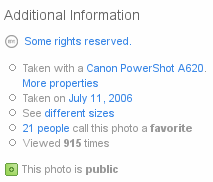
\includegraphics[width=\marginparwidth]{scrsh_flickr_photo_detail_metadata}
  \label{figure:scrsh.flickr.photo.detail.metadata}
}

Flickr is a photo sharing site which are known to be on the cutting edge when
it comes to enabling new and innovating features in it's domain. Flickr has a
quite peculiar history as it started out as a massively multiplayer online
game. An environment for photo sharing within the game was added in 2004 wich
quickly became more popular than the game itself. The focus of the company was
shifted and their new photo sharing community was bought by Yahoo! Inc. in
March 2005 \citep[p.~257]{livingston07}.

This subsequent
analysis of Flickr will be carried out as a registered user. One has to be
registered for interacting with the site in such a way that one leaves
persistent traces. The site has a open nature enabling anonymous access
to the majority of content.

\subsection{Thumbnails}

Already on the welcome page (Figure~\ref{figure:scrsh.flickr.welcome},
p.~\pageref{figure:scrsh.flickr.welcome})
we're finding navigation links that are social of
nature. Four thumbnails functions as sample of the most recently uploaded
photos by other members of the community. One can either navigate straight to
a detailed page for each particular photo by clicking on the respective
thumbnail (Id 6, p.~\pageref{table:flickr.content.inventory.6})
or the profile of the uploader by clicking on their user
name (Id 7, p.~\pageref{table:flickr.content.inventory.7}). Such thumbnails
with minimal meta data (the uploader) are prevalent all over Flickr. Of the
120 pages we collected in our content inventory 26 of them contained
thumbnails. Most of these thumbnails
are giving users incentives to navigate using social means%
\sidefill
\sidenote{Apart from the few pages that only show a
          stream of your own thumbnails--when you're browsing your
          own photos by various methods.}.
Which photos these thumbnails portray is dynamic. That is to say that other
users' actions--uploading a photo, tagging a photo, taking a photo with a
specific camera, collecting photos into sets, and adding photos to a certain
group--all determine the navigational choices you as a user is
presented with.

\subsection{Meta-data}

We arrive on a photo detail page as in
Figure~\ref{figure:scrsh.flickr.photo.detail}
(p.~\pageref{figure:scrsh.flickr.photo.detail})
if we utilize one of these thumbnails for navigation. In addition to comments
on the photo we find meta-data as in 
Figure~\ref{figure:scrsh.flickr.photo.detail.metadata}
(p.~\pageref{figure:scrsh.flickr.photo.detail.metadata}).
Meta-data include the date the photo was taken, the manufacturer and the model
of the camera that was used which are all so called Exif%
\sidenote{Exchangeable Image File: a specification for image file format used
in digital cameras.}
data. Flickr utilize this data by enabling navigation based both on the
dates a picture was taken and by camera make and model. Say you're trying to
find a picture from your home town on a particularly beautiful summer day. By
using date of picture taking based navigation coupled with tags or
geographical data (which both will be discussed shortly) you're probably
increasing you chances of finding what you want. Camera make information could
be useful when looking at the quality of pictures taken with certain cameras
before purchasing one yourself.

\begin{figure}[b]
  \captionstyle{\raggedright}
  \centering
  \strictpagechecktrue
  \begin{adjustwidth*}{0em}{-\wholemargin}
    \begin{minipage}[t]{0.475\wholewidth}
      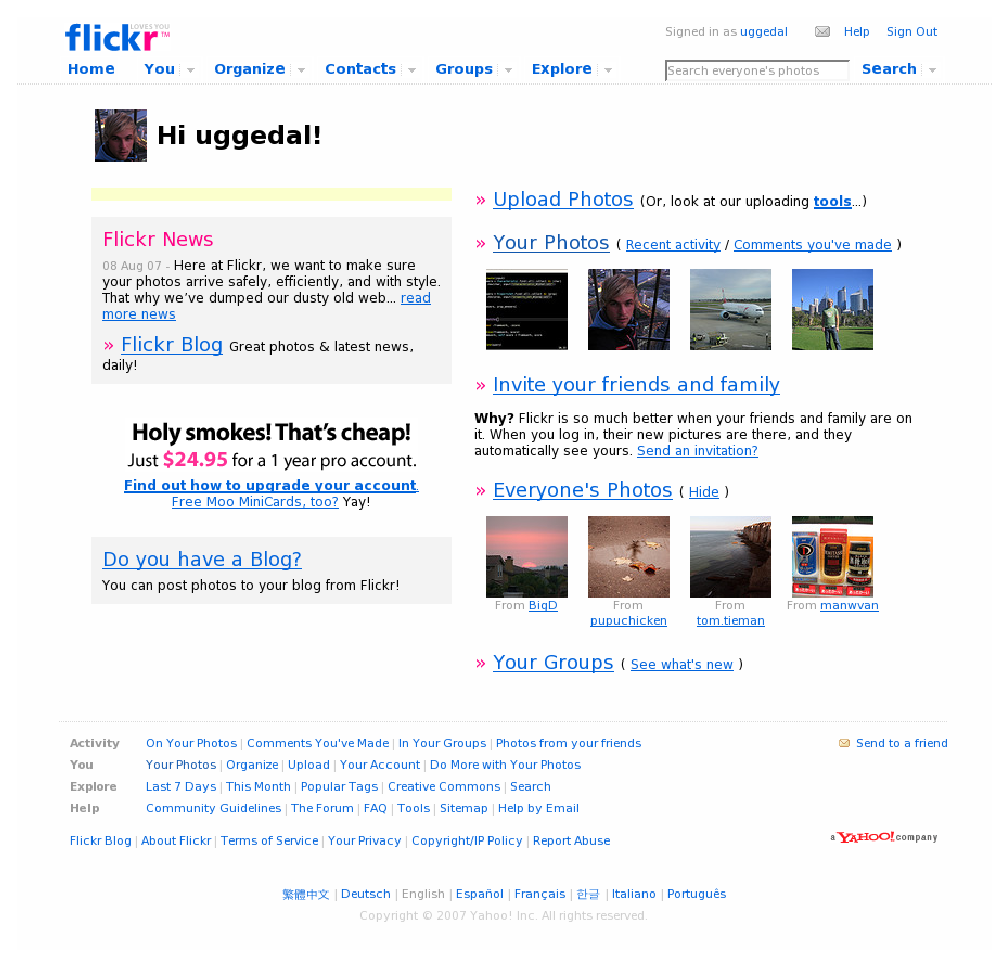
\includegraphics[width=\textwidth]{scrsh_flickr_welcome}
      \caption[Flickr Welcome Page]{%
         The Welcome Page,
         retrieved October 16, 2007, from \url{http://flickr.com}.}
      \label{figure:scrsh.flickr.welcome}
    \end{minipage}
    \hfill
    \begin{minipage}[t]{0.475\wholewidth}
      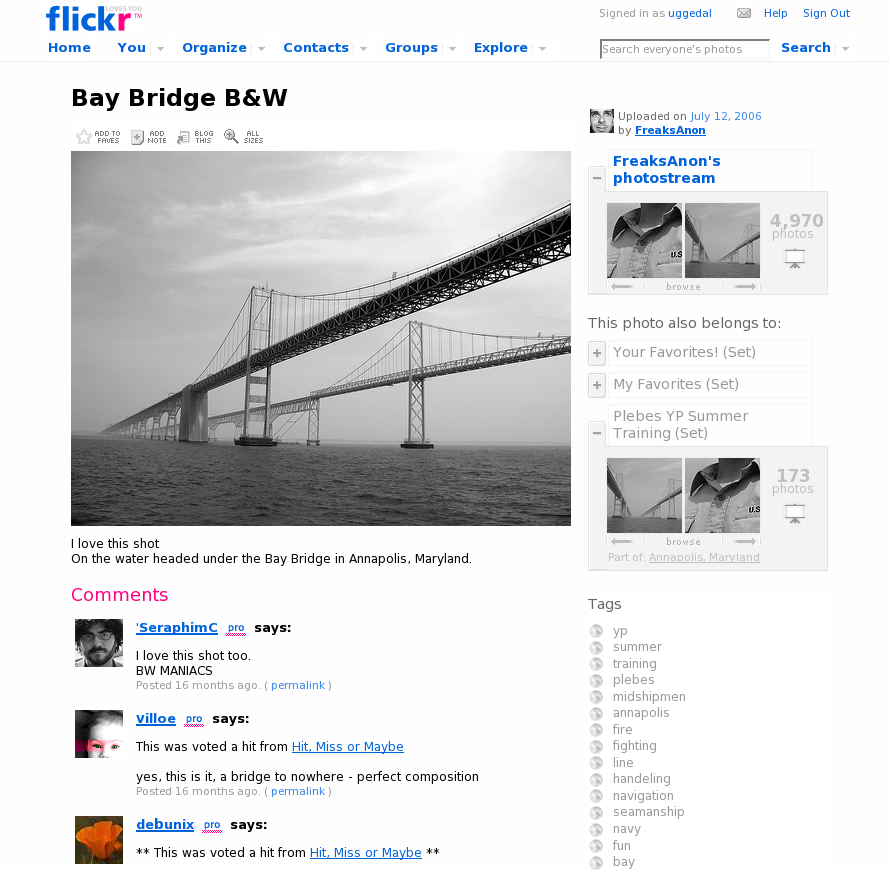
\includegraphics[width=\textwidth]{scrsh_flickr_photo_detail}
      \caption[Flickr Photo Detail Page]{%
         A Photo Detail Page,
         retrieved October 26, 2007, from
         \url{http://flickr.com/photos/benbengraves/187609810}.}
      \label{figure:scrsh.flickr.photo.detail}
    \end{minipage}
  \end{adjustwidth*}
  \normalcaption
\end{figure}

\subsection{Folksonomy}
Of most importance
for Flickr, and indeed what makes Flickr a folksonomy, is it's tagging
abilities. Caterina Fake, cofounder of Flickr, explains it's importance:
``Tagging really revolutionized the way the product behaved.''
\citep[p.~261]{livingston07}
All
registered user can label anyone's photos by applying such short descriptive
tags. This collaborative process lay the ground work for other user's ability
to easily browse photos by topic.
Figure~\ref{figure:scrsh.flickr.tagcloud}
(p.~\pageref{figure:scrsh.flickr.tagcloud}) exemplifies how the user generated
data trough tagging can be used as a navigational aid. A so called \emph{tag
cloud} is used to visualize the popularity (and thereby importance) of the
individual tags. The larger the tag title, the more frequent the tag has been
applied to photographs.

Tag clustering was released in the fall of 2005 \citep{butterfield05} as a way
to easier se the relationships between seperate tags. For any given tag a
cluster of three related tags is generated and displayed to users when they
are browsing as seen in
Figure~\ref{figure:scrsh.flickr.photo.detail}
(p.~\pageref{figure:scrsh.flickr.photo.detail}). Flickr algoritmally generates
these listings based on what tags users tend to use together for labeling a
photo.

Tagging is a very flexible approach only hindered by users' imagination. In the
early days of Flickr there was no support for geographical data. Users soon
found a remedy for this by tagging photos with longitude and latitude. By
using the same technology we're using in our prototype application
(Greasemonkey) they were able to integrate Google Maps%
\sidenote{
  Available at \url{http://maps.google.com}
} in Flickr, enabeling user's to place their photos on a map and automatically
generate geographical coordinate tags%
\sidenote{
  More info about the early days of \emph{geotagging} can be found on the
  remains of the Flickr Geotagging group, available at
  \url{flickr.com/groups/geotagging/}.
}.

\subsection{Geographical data}

In late August 2006 Flickr introduced geotagging abilities
\citep{butterfield06} by integrating mapping aspects from Yahoo! Maps%
\sidenote{
  Available at \url{http://maps.yahoo.com}.
}
Users could now place their photos on a
map to signify where they were captured.
% Finish description.
% Take screenshot.
% Write about the new places feature.
% Write and cite when proper geo data was incorporated.

\subsection{Interestingness}
% Cite collaborative filtering. Introduced in same blog post as clustering.

\begin{figure}[b]
  \centering
  \strictpagechecktrue
  \begin{adjustwidth*}{0em}{-\wholemargin}
    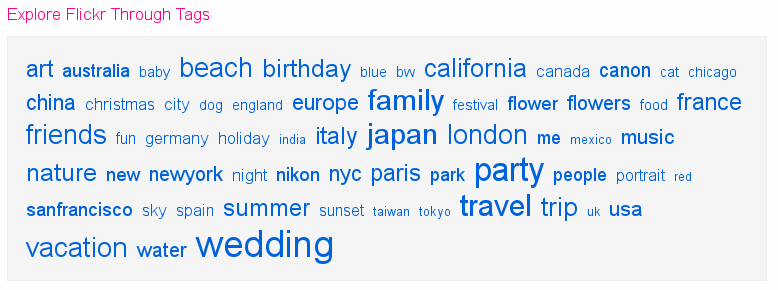
\includegraphics[width=\wholewidth]{scrsh_flickr_tagcloud}
    \caption[Flickr Tag Cloud]{%
       Tag Cloud,
       retrieved November 1, 2007, from \url{http://flickr.com/explore}.}
    \label{figure:scrsh.flickr.tagcloud}
  \end{adjustwidth*}
\end{figure}

\begin{figure}[b]
  \centering
  \strictpagechecktrue
  \begin{adjustwidth*}{0em}{-\wholemargin}
    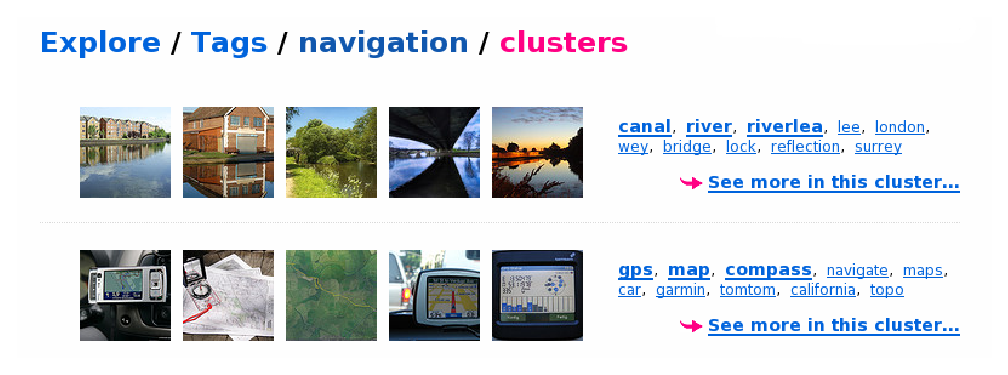
\includegraphics[width=\wholewidth]{scrsh_flickr_tagcluster}
    \caption[Flickr Tag Cluster]{%
       Tag Cloud,
       retrieved November 19, 2007, from
       \url{http://flickr.com/photos/tags/navigation/clusters/}.}
    \label{figure:scrsh.flickr.tagcluster}
  \end{adjustwidth*}
\end{figure}


    \chapter{Reference Test}
    Here is some textual citation of \citet{bush45}.

    Here is a paranthesized citation of \citep{dieberger97}.

    Here is some textual citation of \citet{dieberger00} and the same
    citation with all authors' names included \citet*{dieberger00}.

    Here is a textual citation of several sources
    \citet{dourish94,golder05}.

    Here is some paranthesized citation of \citet{hill92} and the same
    citation with all authors' names included \citet*{hill92}.

    Here is a paranthesized citation of several sources
    \citep{hill94,ohalloran07}.

    Here is a paranthesized citation with additional prefix text
    \citep[online from]{places07}.

    Here we just retrieve the author of a citation \citeauthor{wexelblat99}.

    \begin{appendices}
      \chapter{Content Inventory}

When gathering data in the inventory phase of content analysis the root
document, the main portal to the site under investigation, was entered and
identified in an inventory table with an identifier of \emph{0}. From this
page all relevant navigational links were followed in a logical order (from
top to bottom and left to right on each page). Each new page entered by
following such links was noted down in the inventory table and given an
identifier based on it's hierarchical nature of the navigation system.

The result of this exercise were a table identifying a website's various pages
and the relationships amongst them. To better understand these relationships
content maps based on the raw data from the inventory phase were created
(Appendix~\ref{appendix:content.mapping},
p.~\pageref{appendix:content.mapping}).

\label{appendix:content.inventory}

\section{Flickr}

The following content inventory detailed in
Table~\ref{table:flickr.content.inventory}
(p.~\pageref{table:flickr.content.inventory})
represents the state of the Flickr service as of the 20th of September 2007.
Details could very well have changed since then as
services like these are known to have a rapid development cycle
where changes often are imposed on the user base at quite
a frequent rate.

When collecting data one notices that there is an enormous amount of pages
sharing a common structure only differing in a single or a few variables.
Examples include the user in question for a profile page, the tag for a
listing of photos annotated with such a tag, the date for time based history
listings and so on. I therefore introduced several such variables prefixed
with a dollar sign:
\emph{\$}\footnote{Inspired from variable usage inUNIX shell scripting}.
A complete listing of such variables and their meaning can be found in
Table~\ref{table:flickr.variable.list}
(p.~\pageref{table:flickr.variable.list})

\begin{table}
  \begin{center}
    \begin{small}

      \caption{Variable Listing for Flickr}
      \label{table:flickr.variable.list}

      \begin{tabular}{lp{8cm}}

        \toprule
        Variable & Description \\
        \midrule

        \var{user} &
        Unique nick-name for a user \\

        \var{photo-id} &
        Unique numerical identifier for a photo \\

        \var{photo-title} &
        Textual title of a photo \\

        \var{set-id} &
        Unique numerical identifier for a set (of photos) \\

        \var{set-title} &
        Textual title of a set (of photos) \\

        \var{tag} &
        Unique name for a tag \\

        \var{group} &
        Unique textual name for a group \\

        \var{camera-make} &
        Manufacturer of digital cameras \\

        \var{camera-model} &
        Model number of a particular digital camera \\

        \var{date} &
        A given date (year, optional month, and optional day) \\

        \var{topic-id} &
        Unique numerical identifier for a discussion topic \\

        \var{topic-title} &
        Textual title of a discussion topic \\

        \var{member-count} &
        Variable number of members of a group \\

        \bottomrule

      \end{tabular}
    \end{small}
  \end{center}
\end{table}

% describe the table columns

% Include this after the data has been cleaned up (use best of h1/title).
%
% Most pages have both a title displayed in the browsers title-bar (using a
% HTML title anchor inside the head anchor) and a in page-heading (usually inside
% a HTML h1 anchor). During the content inventory I took not of the most
% descriptive of these two in the following ``Page Title'' columns. There were
% occasions where one of these were lacking in properly describing the pages
% content. Since the aim of this content inventory is to get an informed picture
% of the navigational structures I simply selected the most fitting title.
% I opted to ignore noting down such inconsistencies as one probably would to
% when using content inventory as a tool for improving site architecture.


\setlength\LTleft{0pt plus 1fill minus 1fill}
  \let\LTright\LTleft

% Long multi-page table
\begin{landscape}
  \begin{small}
    \label{table:flickr.content.inventory.1}
    \begin{longtable}{rp{3cm}p{3cm}p{3cm}}
      \caption{Content Inventory of Flickr} \\

  % First page header
  \toprule
  Id & Page Title & Link Name & Link Location \\
  \midrule
  \endfirsthead

  % Remaining pages header
  \caption[]{(continued)}\\
  \toprule
  Id & Page Title & Link Name & Link Location \\
  \midrule
  \endhead

  % Footer except for last page
  \midrule
  \multicolumn{4}{l}{{Continued on Next Page\ldots}} \\
  \endfoot

  % Last page footer
  \bottomrule
  \endlastfoot

  % Data

0 &
Welcome to Flickr &
&
\\
% /

1 &
Photos from \var{user} &
You &
Global navigation \\
% /photos/\var{user}

  1.1 &
  \var{photo-title} &
  Photo thumbnail &
  Content area \\
  % /photos/\var{user}/\var{photo-id}

    1.1.1 &
    Photos from \var{user} &
    \var{user} &
    Content (comments list) \\
    % /photos/\var{user}

    1.1.2 &
    \var{set-title} - a photoset on Flickr &
    \var{set-title} (Set) &
    Right sidebar \\
    % /photos/\var{user}/sets/\var{set-id}

    1.1.3 &
    \var{group} Pool &
    \var{group} (Pool) &
    Right sidebar \\
    % /groups/\var{group}/pool

    1.1.4 &
    \var{user} photos tagged with \var{tag} &
    \var{tag} &
    Right sidebar (tag list) \\
    % /photos/\var{user}/tags/\var{tag}

      1.1.4.1 &
      Photos tagged with \var{tag} &
      public photos tagged with \var{tag} &
      Left sidebar \\
      % /photos/tags/\var{tag}

    1.1.5 &
    Explore your geotagged photos on a Map &
    (map) -> View \var{user} map &
    Right sidebar (details list) \\
    % /photos/\var{user}/\var{photo-id}/map/?view=users

    1.1.6 &
    Explore everyone's geotagged photos on a Map &
    (map) -> see more photos here &
    Right sidebar (details list) \\
    % /photos/\var{user}/\var{photo-id}/map/?view=everyone

    1.1.7 &
    Camera Finder: \var{camera-model} &
    \var{camera-model} &
    Right sidebar (detail list) \\
    % /cameras/\var{camera-make}/\var{camera-model}

    1.1.8 &
    Archive of your photos taken on \var{date} &
    \var{camera-model} &
    Right sidebar (detail list) \\
    % /photos/\var{user}/archives/date-taken/\var{date}

  1.2 &
  \var{set-title} - a photoset on Flickr &
  \var{set-title} &
  Left sidebar \\
  % /photos/\var{user}/sets/\var{set-id}

  1.3 &
  \var{user} sets on Flickr &
  Sets &
  Local navigation \\
  % /photos/\var{user}/sets

    1.3.1 &
    \var{set-title} - a photoset on Flickr &
    \var{set-title} &
    Content area \\
    % /photos/\var{user}/sets/\var{set-id}

      1.1.1.1 &
      \var{photo-title} &
      Photo thumbnail &
      Content area \\
      % /photos/\var{user}/\var{photo-id}/in/set-\var{set-id}

  1.4 &
  \var{user} tags &
  Tags &
  Local navigation \\
  % /photos/\var{user}/tags

    1.4.1 &
    \var{user} photos tagged with \var{tag} &
    \var{tag} &
    Content (tag cloud) \\
    % /photos/\var{user}/tags/\var{tag}

      1.4.1.1 &
      Photos tagged with \var{tag} &
      public photos tagged with \var{tag} &
      Left sidebar \\
      % /photos/tags/\var{tag}

      1.4.1.2 &
      \var{photo-title} &
      Photo thumbnail &
      Content area \\
      % /photos/\var{user}/\var{photo-id}


  1.5 &
  Explore your geotagged photos on a Map &
  Map &
  Local navigation \\
  % /photos/\var{user}/map

    1.5.1 &
    \$photo-name &
    Photo count icon &
    Map \\
    % /photos/\var{user}/map

      1.5.1.1 &
      \var{user} photos tagged with \var{tag} &
      \var{tag} &
      In-line dialog \\
      % /photos/\var{user}/tags/\var{tag}

      1.5.1.2 &
      \var{photo-title} &
      View photo page &
      In-line dialog \\
      % /photos/\var{user}/\var{photo-id}

  1.6 &
  Archive of all your photos on Flickr &
  Archives &
  Local navigation \\
  % /photos/\var{user}/archives

    1.6.1 &
    Archive of your photos taken on \var{date} &
    \var{date} &
    Content area (Taken on) \\
    % /photos/\var{user}/archives/date-taken/\var{date}

      1.6.1.1 &
      \var{photo-title} &
      Photo thumbnail &
      Content area \\
      % /photos/\var{user}/\var{photo-id}

    1.6.2 &
    Archive of your photos posted on \var{date} &
    \var{date} &
    Content area (Posted on) \\
    % /photos/\var{user}/archives/date-posted/\var{date}

      1.6.2.1 &
      \var{photo-title} &
      Photo thumbnail &
      Content area \\
      % /photos/\var{user}/\var{photo-id}

  1.7 &
  \var{user} favorite photos on Flickr &
  Favorites &
  Local navigation \\
  % /photos/\var{user}/favorites

    1.7.1 &
    \var{photo-title} &
    Photo thumbnail &
    Content area \\
    % /photos/\var{user}/\var{photo-id}

  1.8 &
  \var{user} most popular photos, interestingness &
  Popular &
  Local navigation \\
  % /photos/\var{user}/popular-interesting

    1.8.1 &
    \var{photo-title} &
    Photo thumbnail or photo title &
    Content area \\
    % /photos/\var{user}/\var{photo-id}

    1.8.2 &
    \var{user} most popular photos, views &
    Views &
    Sub local navigation \\
    % /photos/\var{user}/popular-views

      1.8.2.1 &
      \var{photo-title} &
      Photo thumbnail or photo title &
      Content area \\
      % /photos/\var{user}/\var{photo-id}

    1.8.3 &
    \var{user} most popular photos, favorites &
    Views &
    Sub local navigation \\
    % /photos/\var{user}/popular-faves

      1.8.3.1 &
      \var{photo-title} &
      Photo thumbnail or photo title &
      Content area \\
      % /photos/\var{user}/\var{photo-id}

    1.8.2 &
    \var{user} most popular photos, comments &
    Comments &
    Sub local navigation \\
    % /photos/\var{user}/popular-comments

      1.8.2.1 &
      \var{photo-title} &
      Photo thumbnail or photo title &
      Content area \\
      % /photos/\var{user}/\var{photo-id}

  1.9 &
  \var{user} &
  Profile &
  Local navigation \\
  % /people/\var{user}

    1.9.1 &
    Photos from \var{user} &
    \var{user} &
    Content (Groups) \\
    % /photos/\var{user}

    1.9.2 &
    \var{group} &
    \var{group} &
    Content (Groups) \\
    % /groups/\var{group}

2 &
Organize your photos &
Organize &
Global navigation \\
% /photos/organize

3 &
Photos from your contacts &
Contacts &
Global navigation \\
% /photos/friends

  3.1 &
  \var{photo-title} &
  Photo thumbnail &
  Content area \\
  % /photos/\var{user}/\var{photo-id}

  3.2 &
  Photos from \var{user} &
  \var{user} &
  Content area \\
  % /photos/\var{user}

4 &
Groups &
Groups &
Global navigation \\
% /groups

  4.1 &
  \var{group} &
  \var{group} &
  Content \\
  % /groups/\var{group}

    4.1.1 &
    \var{group} discussion topics &
    Discussion &
    Local navigation \\
    % /groups/\var{group}/discuss

      4.1.1.1 &
      \var{topic-title} in \var{group} &
      \var{topic-title} &
      Content (topic list) \\
      % /groups/\var{group}/discuss/\var{topic-id}

      4.1.1.2 &
      Photos from \var{user} &
      \var{user} &
      Content (topic list) \\
      % /photos/\var{user}

    4.1.2 &
    \var{group} Pool &
    Pool &
    Local navigation \\
    % /groups/\var{group}/discuss

      4.1.2.1 &
      \var{photo-title} &
      Photo thumbnail &
      Content area \\
      % /photos/\var{user}/\var{photo-id}/in/pool-\var{group}

      4.1.2.2 &
      Photos from \var{user} &
      \var{user} &
      Content area \\
      % /photos/\var{user}

    4.1.3 &
    Explore geotagged photos from \var{group}  &
    Pool &
    Local navigation \\
    % /groups/\var{group}/pool/map?mode=group

      4.1.3.1 &
      \$photo-name &
      Photo count icon &
      Map \\
      % /groups/\var{group}/pool/map?mode=group

        4.1.3.1.1 &
        \var{user} photos tagged with \var{tag} &
        \var{tag} &
        In-line dialog \\
        % /photos/\var{user}/tags/\var{tag}

        4.1.3.1.2 &
        \var{photo-title} &
        View photo page &
        In-line dialog \\
        % /photos/\var{user}/\var{photo-id}

    4.1.3 &
    \var{group}  &
    \var{member-count} Members &
    Local navigation \\
    % /groups\_members.gne?id=\var{group}-id

      4.1.3.1 &
      Photos from \var{user} &
      \var{user} &
      Content area \\
      % /photos/\var{user}

5 &
Explore &
Explore &
Global navigation \\
% /explore

  5.1 &
  \var{photo-title} &
  Photo thumbnail or \var{photo-title} &
  Content (highlighted photo) \\
  % /photos/\var{user}/\var{photo-id}

  5.2 &
  Photos from \var{user} &
  \var{user} &
  Content (highlighted photo) \\
  % /photos/\var{user}

  5.3 &
  Explore interesting photos from the last 7 days &
  last 7 days &
  Content area \\
  % /explore/interesting/7days

    5.3.1 &
    \var{photo-title} &
    Photo thumbnail or \var{photo-title} &
    Content area \\
    % /photos/\var{user}/\var{photo-id}

    5.3.2 &
    Photos from \var{user} &
    \var{user} &
    Content area \\
    % /photos/\var{user}

  5.4 &
  Explore interesting photos from \var{date} &
  \var{date} &
  Content area \\
  % /explore/interesting/\var{date}

    5.4.1 &
    \var{photo-title} &
    Photo thumbnail or \var{photo-title} &
    Content area \\
    % /photos/\var{user}/\var{photo-id}

    5.4.2 &
    Photos from \var{user} &
    \var{user} &
    Content area \\
    % /photos/\var{user}

  5.5 &
  Explore everyones geotagged photos on a Map &
  a map of the world &
  Content area \\
  % /map

    5.5.1 &
    \$photo-name &
    Photo count icon &
    Map \\
    % /map

      5.5.1.1 &
      \var{user} photos tagged with \var{tag} &
      \var{tag} &
      In-line dialog \\
      % /photos/\var{user}/tags/\var{tag}

      5.5.1.2 &
      \var{photo-title} &
      View photo page &
      In-line dialog \\
      % /photos/\var{user}/\var{photo-id}

  5.6 &
  Popular Tags &
  popular tags &
  Content area \\
  % /photos/tags

    5.6.1 &
    Photos tagged with \var{tag} &
    \var{tag} &
    Content (tag cloud) \\
    % /photos/tags/\var{tag}

      5.6.1.1 &
      Photos tagged with \var{tag} &
      Most interesting &
      Left column \\
      % /photos/tags/\var{tag}/interesting

        5.6.1.1.1 &
        \var{photo-title} &
        Photo thumbnail &
        Content area \\
        % /photos/\var{user}/\var{photo-id}

        5.6.1.1.2 &
        Photos from \var{user} &
        \var{user} &
        Content area \\
        % /photos/\var{user}

      5.6.1.2 &
      Photos tagged with \var{tag} &
      \var{tag} clusters &
      Left column \\
      % /photos/tags/\var{tag}/clusters

        5.6.1.2.1 &
        \var{photo-title} &
        Photo thumbnail &
        Content area \\
        % /photos/\var{user}/\var{photo-id}

        5.6.1.2.2 &
        Photos from \var{user} &
        \var{user} &
        Content area \\
        % /photos/\var{user}

        5.6.1.2.3 &
        Photos tagged with \var{tag} &
        \var{tag} &
        Content (cluster list) \\
        % /photos/tags/\var{tag}/clusters

        5.6.1.2.4 &
        Photos tagged with \var{tag} &
        See more of this cluster\ldots &
        Content area \\
        % /photos/tags/\var{tag}/clusters/\var{tag}-\var{tag}-\var{tag}

          5.6.1.2.4.1 &
          \var{photo-title} &
          Photo thumbnail &
          Content area \\
          % /photos/\var{user}/\var{photo-id}

          5.6.1.2.4.2 &
          Photos from \var{user} &
          \var{user} &
          Content area \\
          % /photos/\var{user}

      5.6.1.3 &
      \var{photo-title} &
      Photo thumbnail &
      Content area \\
      % /photos/\var{user}/\var{photo-id}

      5.6.1.4 &
      Photos from \var{user} &
      \var{user} &
      Content area \\
      % /photos/\var{user}

  5.7 &
  Camera Finder &
  Camera finder &
  Content area \\
  % /cameras

    5.7.1 &
    Camera Finder: \var{camera-make} &
    \var{camera-make} &
    Content area \\
    % /cameras/\var{camera-make}

      5.7.1.1 &
      Camera Finder: \var{camera-make}: \var{camera-model} &
      \var{camera-model} &
      Content area \\
      % /cameras/\var{camera-make}/\var{camera-model}

        5.7.1.1.1 &
        \var{photo-title} &
        Photo thumbnail &
        Content area \\
        % /photos/\var{user}/\var{photo-id}

        5.6.1.1.2 &
        Photos from \var{user} &
        \var{user} &
        Content area \\
        % /photos/\var{user}

  5.8 &
  Photos from everyone &
  most recent uploads &
  Content area \\
  % /photos

      5.8.1 &
      \var{photo-title} &
      Photo thumbnail &
      Content area \\
      % /photos/\var{user}/\var{photo-id}

      5.8.2 &
      Photos from \var{user} &
      \var{user} &
      Content area \\
      % /photos/\var{user}

      5.8.3 &
      Popular Tags &
      Popular tags &
      Right sidebar \\
      % /photos/tags

      5.8.4 &
      Creative Commons &
      Creative Commons &
      Right sidebar \\
      % /creativecommons

        5.8.4.1 &
        \var{photo-title} &
        Photo thumbnail &
        Content area \\
        % /photos/\var{user}/\var{photo-id}

        5.8.4.2 &
        Photos from \var{user} &
        \var{user} &
        Content area \\
        % /photos/\var{user}

        5.8.4.3 &
        Photos with Creative Commons \$license-type &
        See more &
        Content (\$license-type) \\
        % /photos/\var{user}

          5.8.4.3.1 &
          \var{photo-title} &
          Photo thumbnail &
          Content area \\
          % /photos/\var{user}/\var{photo-id}

          5.8.4.3.2 &
          Photos from \var{user} &
          \var{user} &
          Content area \\
          % /photos/\var{user}

  5.9 &
  Photos tagged with \var{tag} &
  \var{tag} &
  Content (tag cloud) \\
  % /photos/tags/\var{tag}


  5.10 &
  Explore interesting photos from \var{date} &
  \var{date} &
  Content (A year ago) \\
  % /explore/interesting/\var{date}

    5.10.1 &
    \var{photo-title} &
    Photo thumbnail &
    Content area \\
    % /photos/\var{user}/\var{photo-id}

    5.10.2 &
    Photos from \var{user} &
    \var{user} and see more photos &
    Content area \\
    % /photos/\var{user}

    5.10.3 &
    \var{user} &
    profile &
    Content area \\
    % /people/\var{user}

    5.10.4 &
    Photos tagged with \var{tag} &
    \var{tag} &
    Content area \\
    % /photos/tags/\var{tag}/clusters

  5.11 &
  \var{photo-title} &
  Photo thumbnail or \var{photo-title} &
  Content (A year ago) \\
  % /photos/\var{user}/\var{photo-id}

  5.12 &
  Photos from \var{user} &
  \var{user} &
  Content (A year ago) \\
  % /photos/\var{user}

  5.13 &
  \var{user} &
  profile &
  Content (A year ago) \\
  % /people/\var{user}

  5.14 &
  \var{set-title} - a photoset on Flickr &
  \var{set-title} &
  Content (Sets) \\
  % /photos/\var{user}/sets/\var{set-id}

    5.14.1 &
    \var{photo-title} &
    Photo thumbnail &
    Content area \\
    % /photos/\var{user}/\var{photo-id}/in/set-\var{set-id}

  5.15 &
  Photos from \var{user} &
  \var{user} &
  Content (Sets) \\
  % /photos/\var{user}

  5.16 &
  Groups &
  loads of groups &
  Content (Groups) \\
  % /groups

  5.17 &
  \var{group} &
  \var{group} &
  Content (Groups) \\
  % /groups/\var{group}

  5.18 &
  \var{group} Pool &
  Pool &
  Local navigation \\
  % /groups/\var{group}/pool

  5.19 &
  \var{group}  &
  \var{member-count} Members &
  Local navigation \\
  % /groups\_members.gne?id=\var{group}-id

    \end{longtable}
  \end{small}
\end{landscape}

\section{Amazon}

\section{Facebook}

\section{Del.icio.us}

      \chapter{Content Mapping}

\label{appendix:content.mapping}

A map based approach inspired by Harry Beck's London Underground tube
map seen in Figure~\ref{figure:beck.1933.map}
(p.~\pageref{figure:beck.1933.map})
will be used for visualizing the navigational relationships between content
items. \citet{walsh07} introduced such visualization methods to the information
architecture field.

\begin{figure}[h]
  \begin{center}
    \label{figure:beck.1933.map}
    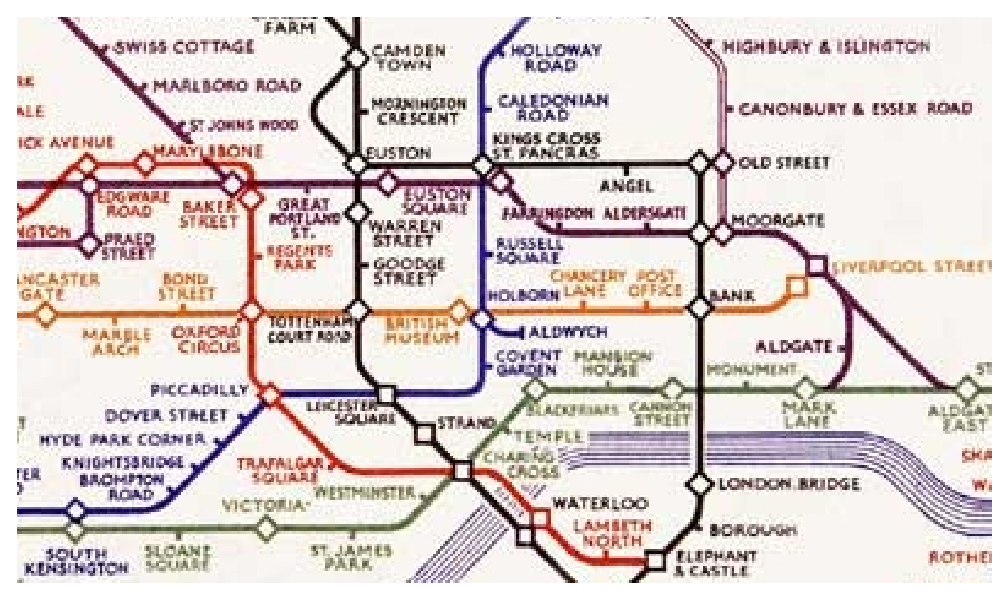
\includegraphics[width=0.9\textwidth]{beck_1933_map}
    \caption[1933 London Underground Tube map]{%
      The present Underground Tube map of London was introduced as early as
      1933 by graphic designer Harry Beck. It's merits are discussed
      in with regards to visual design by \citet{hadlaw03} and highlighted as
      a remarkable example of abstraction in relation to computing by
      \citet{kramer07}. Retrieved from the Transport for London web site:
      \url{http://www.tfl.gov.uk/beckmap1.jpg}.}
  \end{center}
\end{figure}

No maps are available yet since the author don't have access to the required
\emph{Adobe Illustrator} software.

    \end{appendices}
  \backmatter
    \bibliographystyle{apalike}
    \bibliography{bibliography}
\end{document}
